\documentclass[twoside]{article}
\setlength{\oddsidemargin}{0.25 in}
\setlength{\evensidemargin}{-0.25 in}
\setlength{\topmargin}{-0.6 in}
\setlength{\textwidth}{6.5 in}
\setlength{\textheight}{8.5 in}
\setlength{\headsep}{0.75 in}
\setlength{\parindent}{0 in}
\setlength{\parskip}{0.1 in}

\usepackage{graphicx}
\usepackage{url}
\usepackage{mwe}
\usepackage{fancyvrb}


%
% The following commands sets up the lecnum (lecture number)
% counter and make various numbering schemes work relative
% to the lecture number.
%
\newcounter{lecnum}
\renewcommand{\thepage}{\thelecnum-\arabic{page}}
\renewcommand{\thesection}{\thelecnum.\arabic{section}}
\renewcommand{\theequation}{\thelecnum.\arabic{equation}}
\renewcommand{\thefigure}{\thelecnum.\arabic{figure}}
\renewcommand{\thetable}{\thelecnum.\arabic{table}}
\newcommand{\dnl}{\mbox{}\par}

%
% The following macro is used to generate the header.
%
\newcommand{\lecture}[4]{
  \pagestyle{myheadings}
  \thispagestyle{plain}
  \newpage
  \setcounter{lecnum}{#1}
  \setcounter{page}{1}
  \noindent
  \begin{center}
  \framebox{
     \vbox{\vspace{2mm}
   \hbox to 6.28in { {\bf COMPSCI~630~~~Systems
                       \hfill Fall 2019} }
      \vspace{4mm}
      \hbox to 6.28in { {\Large \hfill Lecture #1  \hfill} }
%       \hbox to 6.28in { {\Large \hfill Lecture #1: #2  \hfill} }
      \vspace{2mm}
      \hbox to 6.28in { {\it Lecturer: #3 \hfill Scribe: #4} }
     \vspace{2mm}}
  }
  \end{center}
  \markboth{Lecture #1: #2}{Lecture #1: #2}
  \vspace*{4mm}
}

%
% Convention for citations is authors' initials followed by the year.
% For example, to cite a paper by Leighton and Maggs you would type
% \cite{LM89}, and to cite a paper by Strassen you would type \cite{S69}.
% (To avoid bibliography problems, for now we redefine the \cite command.)
%
\renewcommand{\cite}[1]{[#1]}

% \input{epsf}

%Use this command for a figure; it puts a figure in wherever you want it.
%usage: \fig{NUMBER}{FIGURE-SIZE}{CAPTION}{FILENAME}
\newcommand{\fig}[4]{
           \vspace{0.2 in}
           \setlength{\epsfxsize}{#2}
           \centerline{\epsfbox{#4}}
           \begin{center}
           Figure \thelecnum.#1:~#3
           \end{center}
   }

% Use these for theorems, lemmas, proofs, etc.
\newtheorem{theorem}{Theorem}[lecnum]
\newtheorem{lemma}[theorem]{Lemma}
\newtheorem{proposition}[theorem]{Proposition}
\newtheorem{claim}[theorem]{Claim}
\newtheorem{corollary}[theorem]{Corollary}
\newtheorem{definition}[theorem]{Definition}
\newenvironment{proof}{{\bf Proof:}}{\hfill\rule{2mm}{2mm}}

% Some useful equation alignment commands, borrowed from TeX
\makeatletter
\def\eqalign#1{\,\vcenter{\openup\jot\m@th
 \ialign{\strut\hfil$\displaystyle{##}$&$\displaystyle{{}##}$\hfil
     \crcr#1\crcr}}\,}
\def\eqalignno#1{\displ@y \tabskip\@centering
 \halign to\displaywidth{\hfil$\displaystyle{##}$\tabskip\z@skip
   &$\displaystyle{{}##}$\hfil\tabskip\@centering
   &\llap{$##$}\tabskip\z@skip\crcr
   #1\crcr}}
\def\leqalignno#1{\displ@y \tabskip\@centering
 \halign to\displaywidth{\hfil$\displaystyle{##}$\tabskip\z@skip
   &$\displaystyle{{}##}$\hfil\tabskip\@centering
   &\kern-\displaywidth\rlap{$##$}\tabskip\displaywidth\crcr
   #1\crcr}}
\makeatother

% **** IF YOU WANT TO DEFINE ADDITIONAL MACROS FOR YOURSELF, PUT THEM HERE:



% Some general latex examples and examples making use of the
% macros follow.

\begin{document}

%FILL IN THE RIGHT INFO.
%\lecture{**LECTURE-NUMBER**}{**DATE**}{**LECTURER**}{**SCRIBE**}
\lecture{9}{October 8}{Emery Berger}{Soubhik Rakshit, James Schofield}

\section{Standard exploits}

The Intel x86 instruction set has variable sized instructions. \textit{NOP} is only 1 byte whereas \textit{LOCK, REP} etc. are multiple bytes long. The longest instruction in x86 is 15 bytes long! Variable sized instructions lead to several vulnerabilities which attackers can exploit. Additionally, a wide range of low-level attacks are enabled by the absence of proper memory protection and security.

Some of the exploits discussed in class are:
\begin{itemize}
	\item Buffer overflow
	\item Stack smashing
	\item Return Oriented Programming (ROP)
	\item DDoS attacks
	\item Dangling pointers / Use after free
	\item vtable attack
\end{itemize}

\subsection{Buffer overflow}
Buffer overflow is a common exploit where the attacker's job is to overflow the buffer and write on memory locations that the attacker should not have access to. Thus, the attacker can overflow the buffer and, for instance, overwrite a location where some password is stored. In this way, the attacker can set his own password using buffer overflow. The attacker can also write the payload onto the memory (so-called 'shellcode') with the intent of gaining superuser access to the system (or 'rooting' it). This is shown in Figure \ref{fig:buffer1} and \ref{fig:buffer2}.

In other to ensure that the shellcode is delivered correctly, a bunch of \textit{NOP} (no operation) instructions can be placed in front of it to direct how the section of code will be executed. This is called a \textit{NOP sled}.

\begin{figure}[ht]
	\centering
	\begin{minipage}{0.45\textwidth}
		\centering
		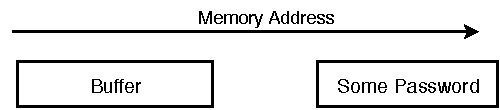
\includegraphics[width=0.8\linewidth]{buffer1} % first figure itself
		\caption{Overwriting password}
		\label{fig:buffer1}
	\end{minipage}\hfill
	\begin{minipage}{0.45\textwidth}
		\centering
		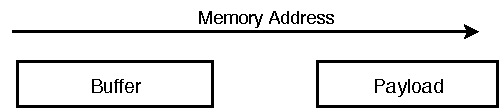
\includegraphics[width=0.8\linewidth]{buffer2} % second figure itself
		\caption{Deploying a payload}
		\label{fig:buffer2}
	\end{minipage}
\end{figure}

\subsection{Stack smashing attack}
Stack smashing is another type of attack where the stack is overwritten and a \textit{JUMP} instruction might actually go to a different location than was intended. A stack is shown in Figure \ref{fig:stack}. If the \textit{JUMP} instruction could be modified, an attacker can execute some other code.
\begin{figure}[h]
\centering
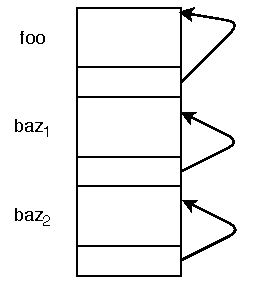
\includegraphics[width=0.25\linewidth]{stack}
\caption{}
\label{fig:stack}
\end{figure}

Another problem is when passing parameters as arguments to a function. If there are multiple parameters, the first few are placed in the registers whereas the others are placed in the stack. Now if an attacker changes the \textit{JUMP} instruction after the parameters in the stack to the Program Counter (PC), then the system is compromised. It might very well be possible to bypass authentication procedures using this technique. 

\subsection{ROP attacks}
ROP attacks are very hard to perform. Here, the attacker does not need to write any explicit code. The attacker finds a large codebase and gathers machine instructions for a shellcode which are scattered throughout the codebase. The machine instructions are stitched together using \textit{JUMP} instructions to perform the operations desired by the attacker. By doing this, it is possible to create an entire shellcode out of an existing completely unrelated program like that of a web browser.

\subsection{DDoS attacks}
In 1988, Robert Morris unexpectedly created the first ever Distributed Denial of Service (DDoS) attack when he created a virus that could infect a computer on the network and use it to replicate to another computer. An infected computer would contact every other computer it could, but it had to functionality to check whether a computer it contacted was already infected. As such, an infected computer would repeatedly send messages to all the computers it could, overwhelming those computers' abilities to receive them or anything else.

DDoS differs from the other forms of attack discussed here in that the attacker doesn't get access to the system. Instead, it focuses on denying any user access to the system, generally by sending overwhelmingly large amounts of information to it.

Other forms of DDoS attacks include SYN Flooding where a client repeatedly sends synchronization packets to every port on a server using a fake IP address.

\newpage
\subsection{Dangling pointers / Use after free}
\begin{VerbatimOut}{later.tex}
	\begin{verbatim}
	x = new(...);
	y = x;
	delete x;
	z = new(...);
	// If z is allocated to the space where
	// y was present, then y can access z.
	print(y);
	\end{verbatim}
\end{VerbatimOut}

        \begin{verbatim}
        x = new(...);
        y = x;
        delete x;
        z = new(...);
        // If z is allocated to the space where
        // y was present, then y can access z.
        print(y);
        \end{verbatim}


Temporal safety is the work of a garbage collector. One of its roles is to prevent this kind of attack.

\subsection{vtable attack}
In C++, a destructor is called when any object is destroyed. The virtual dispatch table (vtable) contains the references for which function to execute when the destructor is called. If the vtable can be overflowed to point to a location where shellcode is stored, then it would be easy for an attacker to execute arbitrary code or root the system.

\section{Preventing attacks}
There are some unique solutions to prevent some of these attacks. However, newer attacks have appeared to attempt to circumvent these defensive measures.

There exists solutions where the system can detect if a \textit{JUMP} leads to execution of shellcode. The system can recognize code which appears suspicious. However, polymorphic shellcode has been developed which is generated dynamically thereby making a system unable to recognize if a code is actual shellcode or not. Also, developers have written shellcode in plain English (ASCII) which makes it very hard to recognize it.

\subsection{Preventing stack smashing attack}
There are several approaches to prevent stack smashing attacks.

\begin{itemize}
	\item Keep multiple copies of the stack. The stack which is not being used is called the shadow stack. For every \textit{JUMP} instruction, compare the return address with the shadow stack.
	\item Stack canaries are also used where known values are placed in the stack. If anytime, those get modified, the system learns that an attack is taking place and stops further execution.
	\item Stacks may be encrypted using keys. An easy and fast way to do it is to XOR the stack value with a known key. Thus whenever, decryption is needed, XOR can be applied with the same key. So, only the key needs to be protected in this case.
\end{itemize}
There are no such protections about the heap. Naturally, copying the heap would be wildly impractical. However, different approaches using randomization and dispersion exist, including Berger's own DieHarder memory management system for the heap.

\subsection{Have executable bits for every file}
Intel at first didn't have executable bits to set. Thus, any user could read any other user's files. This led to a return-to-libs attack where a return address on the call stack is replaced by an address of another function that is already present in the executable memory of the process, bypassing the no-execute-bit feature. Later, Intel implemented executable bits and called it NX\_PROTECTION.

This could also be exploited by using a system function call which could execute a string as a command.

\subsection{Control Flow Integrity}
One approach attempts to ensure control flow integrity (CFI), by ensuring when every jump is made that that jump is in fact legal. WebAssembly, for instance, explicitly preserves CFI. Jumps can only be made to the callers of the function. \textit{Uncontrolled JUMP} does not exist in WebAssembly.

In order to make this possible, \textit{JUMP} instructions must pass through some other function. WEBM does this by using a table. In other words, the problem is solved by adding an additional level of indirection. There is a maxim in CS that all CS problems can be solved by adding a level of indirection. However, this comes at the cost of some speed, leading to the contrary maxim that all CS optimizations can be made by removing a level of indirection.

\subsection{Attacks and Difficulty}
Many of the attacks described would require immense amounts of work to be put into practice, let alone achieve something of value. When many of these exploits were discussed, many of them were dismissed for this very reason. Ultimately, however, the difficulty of the problem didn't stop people from finding out a way to use these exploits. Most of the time, these exploits are used by 'script kiddies' who are using tools they have downloaded from other people. As such, so long as one person takes the time to find and use an exploit, and publish their results, there exists a serious danger.

\section{RISC vs CISC}
A RISC approach uses a smaller instruction set of fixed size. Beyond the previously discussed security benefits of a fixed-sized instruction set, similar sized instructions are easier to pipeline.
The RISC approach had several readily-apparent benefits:
\begin{itemize}
	\item Easier to parse `decode'
	\item Harder to exploit
	\item Faster and easier to design hardware.
\end{itemize}
Ultimately, RISC won because of the benefits of small, uniform instructions, not necessarily because of the benefits of a reduced instruction set. Modern 'RISC' architectures can still have a large instruction set with very specific instructions, as ARM demonstrates. ARM, for instance, has AVX vector instructions and specific cryptography instructions, two very specific groups of instructions. It also has memory protections. 

Google developed ASan (Address Sanitizer) which is a fast memory error detector. However, it slows down program execution. It is good for testing purposes, including in Homework 1.

\section{Very Long Instruction Word}
Very Long Instruction Word (VLIW), as it sounds, is an architecture approach using a combination of many instructions. Ideally, each instruction word should contain a set of instructions, all of which should execute in parallel. While this sounds like an intriguing idea in theory, in reality it proved disastrous. In a pipeline, the entire VLIW instruction has to wait until the each individual instruction has finished. The potential VLIW instruction writer often has absolutely no way to know which instructions will resolve at the same time, meaning that this approach tends to lead to massive slowdowns. Intel attempted their own VLIW infrastructure, known as EPIC/Itanium, during the move from 32 bit to 64 bit. It was an absolute disaster.

Meanwhile, AMD simply created a 64 bit extension to x86 and released it, leading to a rapid increase in their market share, at least until Intel did the same thing.

\section{Concurrency}
Race conditions arise during parallel execution. Depending on scheduling by the OS, reads could have different results if reads and writes are happening simultaneously. This can lead to bizarre unintended behavior, and in many cases should be avoided. There is some controversy in CS if all races are bad, or if there exist 'benign races' which aren't really an issue.

Threads are also known as light weight processes.

Processes have multiple threads, address space (heap, globals, stack), file handles.

Threads have context space to track program counter, instruction pointer and save registers.

All threads use the same stack physically although logically, the stacks are separate.

Some concurrency errors are:
\begin{itemize}
	\item Races
	\item Atomicity violation
	\item Order violation
	\item Deadlock
	\item Livelock
\end{itemize}

Concurrency errors are non-deterministic; in other words, they don't happen on every run of a program. As such, they can often be miserable to debug. Non-deterministic bugs are often referred as Heisenbugs. Somewhat unfairly to Niels Bohr, 'Bohr bugs' are deterministic.

From the perspective of an end user, Heisenbugs tend to be better than deterministic bugs, as the bug can often be solved by rerunning the program. If a bug is fully deterministic, restarting the program will do absolutely nothing. However, it is comparatively much more difficult to debug Heisenbugs, especially if the frequency of the bug is very low.

\end{document}
